\documentclass[tikz,border=4pt]{standalone}
% Shared style for every figure and for the deck: one accent, one
% highlight, thin lines, rounded nodes, nothing decorative.
\usepackage[T1]{fontenc}
\usepackage{lmodern}
\renewcommand{\familydefault}{\sfdefault}
\usepackage{tikz}
\usetikzlibrary{arrows.meta,positioning,calc,shapes.misc,fit,backgrounds,decorations.pathreplacing}
\definecolor{ink}{RGB}{40,40,40}
\definecolor{soft}{RGB}{150,150,150}
\definecolor{faint}{RGB}{225,225,225}
\definecolor{accent}{RGB}{0,95,115}
\definecolor{accentlight}{RGB}{214,232,236}
\definecolor{warn}{RGB}{196,84,40}
\definecolor{warnlight}{RGB}{247,226,216}
\tikzset{
  every picture/.style={color=ink, line width=0.5pt, font=\small},
  node distance=12mm and 18mm,
  box/.style={draw=ink, rounded corners=2pt, fill=white, inner sep=5pt, minimum height=7mm, align=center},
  maker/.style={box, minimum width=18mm},
  cat/.style={box, inner sep=3.5pt, minimum height=6mm},
  root/.style={box, fill=accentlight, draw=accent},
  bad/.style={box, fill=warnlight, draw=warn},
  ghost/.style={box, draw=soft, text=soft, dashed},
  flow/.style={-{Stealth[length=4pt,width=3.5pt]}, line width=0.5pt},
  sub/.style={-{Stealth[length=4pt,width=3.5pt]}, line width=0.5pt, color=soft},
  strong/.style={flow, color=accent, line width=0.8pt},
  wrong/.style={flow, color=warn},
  lbl/.style={font=\footnotesize, text=ink, inner sep=1.5pt, fill=white},
  note/.style={font=\footnotesize, text=soft, align=center},
  rate/.style={font=\footnotesize, text=accent, inner sep=1pt, fill=white},
}

\usepackage{amsmath}
\usepackage{pgfplots}
\pgfplotsset{compat=1.17}

\begin{document}
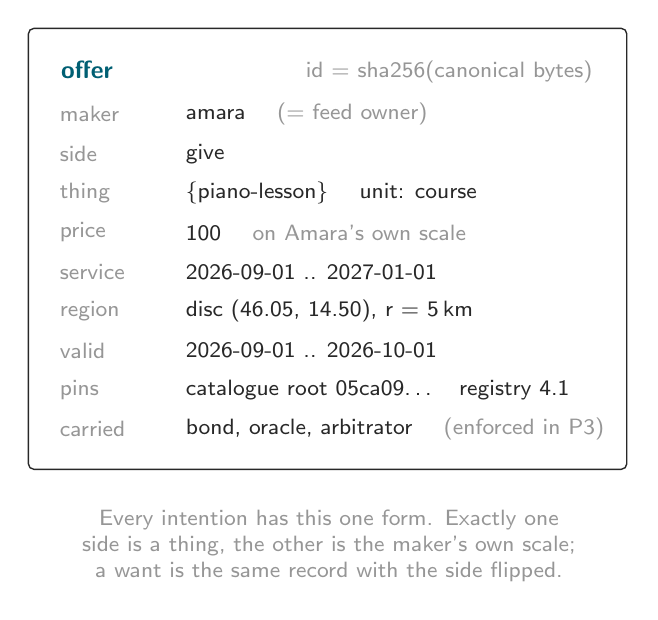
\begin{tikzpicture}[k/.style={anchor=west, font=\footnotesize, text=soft, inner sep=0pt}, v/.style={anchor=west, font=\footnotesize, inner sep=0pt}]
  \node[box, minimum width=76mm, minimum height=56mm, anchor=north west] (card) at (0,0) {};
  \node[anchor=north west, font=\small\bfseries, text=accent] at (3mm,-3mm) {offer};
  \node[anchor=north east, font=\footnotesize, text=soft] at (73mm,-3mm) {id = sha256(canonical bytes)};
  \node[k] at (4mm,-11mm) {maker};   \node[v] at (20mm,-11mm) {amara \quad {\color{soft}(= feed owner)}};
  \node[k] at (4mm,-16mm) {side};    \node[v] at (20mm,-16mm) {give};
  \node[k] at (4mm,-21mm) {thing};   \node[v] at (20mm,-21mm) {\{piano-lesson\} \quad unit: course};
  \node[k] at (4mm,-26mm) {price};   \node[v] at (20mm,-26mm) {100 \quad {\color{soft}on Amara's own scale}};
  \node[k] at (4mm,-31mm) {service}; \node[v] at (20mm,-31mm) {2026-09-01 .. 2027-01-01};
  \node[k] at (4mm,-36mm) {region};  \node[v] at (20mm,-36mm) {disc (46.05, 14.50), r = 5\,km};
  \node[k] at (4mm,-41mm) {valid};   \node[v] at (20mm,-41mm) {2026-09-01 .. 2026-10-01};
  \node[k] at (4mm,-46mm) {pins};    \node[v] at (20mm,-46mm) {catalogue root 05ca09\ldots \quad registry 4.1};
  \node[k] at (4mm,-51mm) {carried}; \node[v] at (20mm,-51mm) {bond, oracle, arbitrator \quad {\color{soft}(enforced in P3)}};
  \node[note, text width=74mm, anchor=north west] at (0,-60mm) {Every intention has this one form. Exactly one side is a thing, the other is the maker's own scale; a want is the same record with the side flipped.};
\end{tikzpicture}
\end{document}
